\section{Durchführung}
\label{sec:Durchführung}


\subsection{Aufbau}
Der Versuchsaufbau besteht aus einer Grundplatte mit vier rechteckigen Stäben, die an einer Seite von einem Peltier-Element simultan geheizt oder gekühlt werden.
Die Stäbe sind aus drei verschiedenen Materialien:  Aluminium, Edelstahl und zweimal Messing, mit verschiedenen Durchmessern.
Zusätzlich sind an jedem Stab zwei Thermoelemente, welche die Temperatur an verschiedenen Stellen der Stäbe messen \autoref{fig:Versuchsaufbau}.
Die Thermoelemente sind verbunden mit einem GLX Datenlogger \autoref{fig:GLX}, welcher die Temperaturen aufnimmt und eine Tabelle überführt.
Zuletzt gibt es auch eine Spannungsquelle, welche bei der statischen Mode eine Betriebspannung von $5\si{V}$ auf das Heizelement überträgt. 
Bei der der dynamischen Mode wird sie auf $8\si{V}$ eingestellt. Bei beidem wird der Strom auf Maximal gestellt.

\begin{figure}[H]
    \centering
    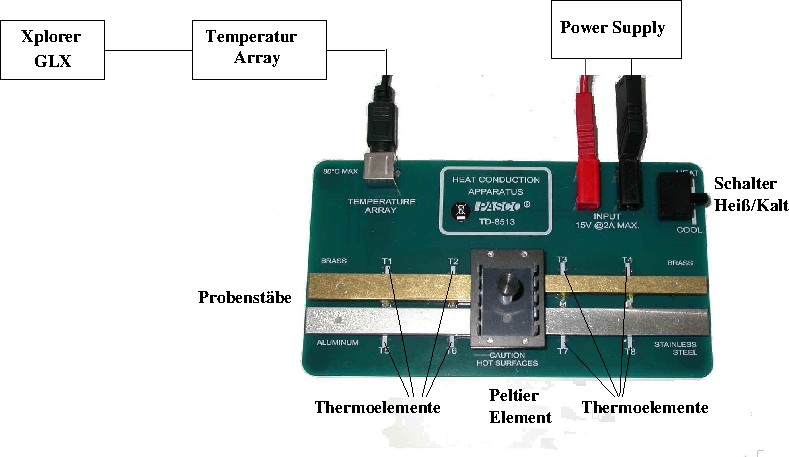
\includegraphics{content/Abb_1.pdf}
    \caption{Grundplatte mit Aluminium, Edelstahl und zweimal Messing\cite[3]{V204}}
    \label{fig:Versuchsaufbau}
\end{figure}

\subsection{Statische Methode}
\label{subsec:durch_stat}
An allen acht Thermoelementen wird der Temperaturverlauf in Abhängigkeit des der Zeit gemessen.
Dafür wird die Abtastrate beim GLX auf $\Delta t_{GLX} = 5\si{s}$ Sekunden gestellt.
Es wird solange gemessen bis das Thermoelement T7 $\qty{45}{\degreeCelsius}$ anzeigt.
Während des Heizvorgangs werden Isolierungen über die Stäbe gelegt, damit der Wärmeaustausch mit der Umgebung verringert wird.
Nach der Messung müssen die Stäbe wieder gekühlt werden, sodass deren Temperaturen maximal $30$ betragen.

\subsection{Dynamische Methode}
\label{subsec:durch_dyn}
Ein andere Name für dieses Methode ist die Angström-Messverfahren.
Dabei werden die Probenstäbe periodisch geheizt.
Die Abtastrate wird vorher auf $\Delta t_{GLX} = 2\si{s}$ geändert.\\
Die erste Messung ist über eine Periode von $80\si{s}$, wobei die ersten $40\si{s}$ geheizt und die letzten $40\si{s}$ gekühlt wird.
Während gekühlt wird muss das Peltier-Element auf "COOL" gestellt werden und die Wärmeisolatoren werden abgenommen.
Diese Messung geht über $10$ Perioden.\\
Die zweite Messung wird analog durchgeführt. 
Die Periode beträgt nun jedoch $200 \si{s}$ und die Messung endet, wenn eines der Thermoelemente $\qty{80}{\degreeCelsius}$ erreicht.

\begin{figure}[H]
    \centering
    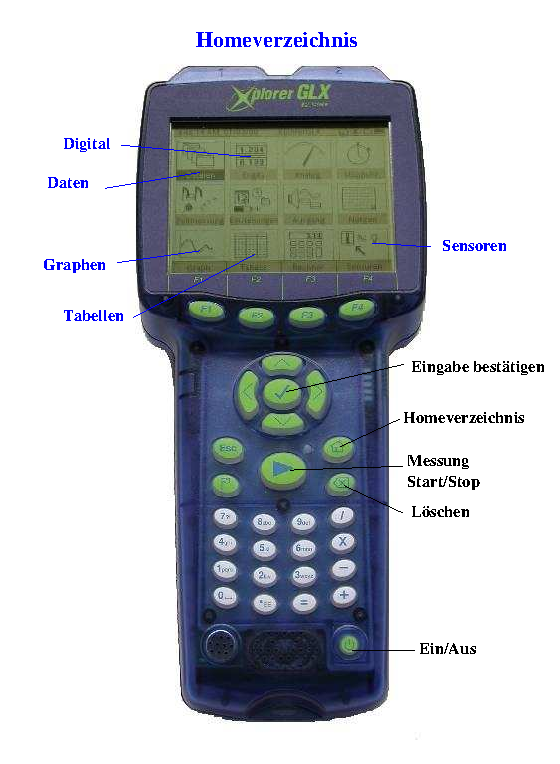
\includegraphics{content/Abb_2.pdf}
    \caption{Xplore GLX\cite[5]{V204}}
    \label{fig:GLX}
\end{figure}

T1 Messing dick fern
T2 Messing dick nah
T3 Messing dünn nah 
T4 Messing dünn fern
T5 Aluminium fern
T6 Aluminium nah
T7 Edelstahl nah
T8 Edelstahl fern